\documentclass[11pt,aspectratio=169]{beamer}
\usepackage{amsmath,amssymb,booktabs,array,graphicx,tikz,listings,lmodern}
\usetikzlibrary{arrows.meta,positioning,calc}
\newcolumntype{P}[1]{>{\raggedright\arraybackslash}p{#1}}
\setlength{\tabcolsep}{3pt}
\usefonttheme{professionalfonts}
\definecolor{Navy}{HTML}{15324F}
\definecolor{Teal}{HTML}{007F86}
\definecolor{Gold}{HTML}{DAA641}
\definecolor{Red}{HTML}{BC4141}
\definecolor{Muted}{HTML}{586B7A}
\definecolor{Pale}{HTML}{F1F5F7}
\setbeamercolor{normal text}{fg=Navy,bg=white}
\setbeamercolor{structure}{fg=Teal}
\setbeamercolor{frametitle}{fg=Navy,bg=white}
\setbeamercolor{alerted text}{fg=Red}
\setbeamercolor{block title}{fg=white,bg=Teal}
\setbeamercolor{block body}{fg=Navy,bg=Pale}
\setbeamertemplate{navigation symbols}{}
\setbeamertemplate{itemize item}{\color{Teal}\scriptsize$\blacktriangleright$}
\setbeamertemplate{itemize subitem}{\color{Teal}\tiny$\bullet$}
\setbeamertemplate{frametitle}{\vspace{3mm}\insertframetitle\par\vspace{1mm}{\color{Teal}\rule{\textwidth}{.6pt}}}
\setbeamertemplate{footline}{\hspace{9mm}\color{Muted}\scriptsize Spatially Abled\hfill GeoResilient\hspace{4mm}\insertframenumber\,/\,\inserttotalframenumber\hspace{9mm}\vspace{3mm}}
\setbeamerfont{frametitle}{size=\Large,series=\bfseries}
\setbeamersize{text margin left=9mm,text margin right=9mm}
\setbeameroption{hide notes}
\newcommand{\src}[1]{\vfill{\fontsize{7.5}{9}\selectfont\color{Muted}#1\par}}
\newcommand{\takeaway}[1]{\par\vspace{2mm}{\color{Teal}\bfseries #1\par}}
\newcommand{\img}[2]{\includegraphics[width=\linewidth,height=#2,keepaspectratio]{assets/#1}}
\newcommand{\smallitems}{\setlength{\itemsep}{1.5mm}}
\lstset{basicstyle=\ttfamily\small,breaklines=true,columns=fullflexible,keepspaces=true,frame=single,
        rulecolor=\color{Teal},backgroundcolor=\color{Pale},showstringspaces=false}
% Values derived from local saved outputs by build_assets.py
\newcommand{\MeanUniformLoss}{23.51}
\newcommand{\MeanPopulationLoss}{30.84}
\newcommand{\PninetyUniformLoss}{27.27}
\newcommand{\PninetyPopulationLoss}{41.09}
\newcommand{\UniformConnectivity}{99.9349}
\newcommand{\PopulationConnectivity}{99.9154}
\newcommand{\PopulationRetained}{99.9566}
\newcommand{\ExpectedCutOff}{0.019531}
\newcommand{\ExampleComposite}{0.8715}
\newcommand{\WestVuln}{22.06}
\newcommand{\EastVuln}{25.68}
\newcommand{\CriticalRows}{11 & 4.14 & 11.17\\
10 & 4.14 & 9.30\\
9 & 4.14 & 7.49\\
}

\title{GeoResilient}
\subtitle{An Open GIS Framework for Assessing the Structural Resilience of Urban Road Networks}
\author{Spatially Abled}
\date{13 October 2026}
\hypersetup{pdftitle={GeoResilient - Mid-evaluation},pdfauthor={Spatially Abled},pdfsubject={Spatial Informatics: Tiers 1 and 2}}

\begin{document}

% 01
\begin{frame}[plain]
\vspace{3mm}
{\color{Muted}\large Spatial Informatics\hfill Mid-evaluation\par}
\vspace{4mm}
{\fontsize{30}{36}\selectfont\bfseries\color{Navy}GeoResilient\par}
\vspace{3mm}
{\Large An Open GIS Framework for Assessing the\par Structural Resilience of Urban Road Networks\par}
\vspace{3mm}
{\color{Teal}Proposed case study: Hyderabad, India\par}
\vspace{3mm}
{\color{Teal}\rule{\textwidth}{1pt}}\par
\vspace{3mm}
{\large\bfseries Spatially Abled\par}
\vspace{2mm}
{\small Dombu Pawar \enspace$\cdot$\enspace Papa Mahtele\par
Dev Birenkumar Pravinchandra Patel\par
Nimalan Bharathi \enspace$\cdot$\enspace Manoj Gupta\par}
\vfill
{\small Tiers 1--2: network structure, disruption analysis and population weighting\hfill 13 October 2026\par}
\note{Introduce the project and team. Hyderabad is the proposed application, while the results shown today are controlled demonstrations and documented earlier validation.}
\end{frame}

\section{Problem statement}
% 02
\begin{frame}{Problem statement}
\begin{itemize}\smallitems
\item A dense road map can hide dependence on a few bridges, corridors or junctions.
\item Closing one important road can lengthen routes, isolate areas and reduce accessibility.
\item Topological damage and the impact on population can point to different priorities.
\item We need reproducible metrics and maps to identify critical roads, vulnerable nodes and affected zones.
\end{itemize}
\takeaway{Assess how a road network performs when its physical roads fail.}
\src{Source: GeoResilient project proposal, pp. 1--3. The mid-evaluation addresses structural and population-based measures.}
\note{Explain why counting roads or looking at a map is insufficient. The current framework assesses structural disruption; it does not yet model emergency-service demand or traffic.}
\end{frame}

% 03
\begin{frame}{A single connecting road can dominate connectivity}
\centering\img{problem_schematic.pdf}{4.4cm}
\begin{itemize}\setlength{\itemsep}{1.5mm}
\item Local street density does not guarantee an alternative route between districts.
\item Criticality measures the consequence of closure; reliability also considers its probability.
\end{itemize}
\src{Illustrative topology, not an observed Hyderabad network. Motivation: Albert et al. (2000); Taylor et al. (2006).}
\end{frame}

% 04
\begin{frame}{Mid-evaluation scope: Tiers 1 and 2}
\begin{columns}[T,totalwidth=\textwidth]
\column{.49\textwidth}
\textbf{Tier 1: the road graph}
\begin{itemize}\smallitems
\item Cleaning and centralities
\item Redundancy and critical roads
\item Attack versus random failure
\item Connectivity and distance accessibility
\item Travel-time reliability when data permit
\end{itemize}
\column{.47\textwidth}
\textbf{Tier 2: population and zones}
\begin{itemize}\smallitems
\item Allocate population to graph nodes
\item Compute population variants
\item Aggregate results by supplied polygons
\item Produce maps, rankings and a scorecard
\end{itemize}
\end{columns}
\takeaway{Tickets 01--15 have implementations; Ticket 15 reports a validation mismatch.}
\src{Scope agreed for mid-evaluation; plan/DESIGN.md and TICKET\_UPDATES.md. Facilities, traffic modelling and Ticket 16 are later work.}
\end{frame}

\section{Data used}
% 05
\begin{frame}{Data used and their role}
\small
\renewcommand{\arraystretch}{1.12}
\begin{tabular}{P{3.4cm}P{9.5cm}}
\toprule
\textbf{Input} & \textbf{Role in the framework}\\
\midrule
OpenStreetMap & Road topology, geometry, directions and attributes via OSMnx\\
WorldPop & 100 m population counts, clipped and allocated to nodes\\
Zone polygons & Polygon IDs and names for reporting by administrative area\\
Published city graphs & Original topology and road lengths for literature validation\\
Synthetic networks & Controlled graphs and count rasters with known answers\\
\bottomrule
\end{tabular}
\vspace{3mm}
\small Failure probabilities: user-supplied when available; length proxy otherwise.
\src{Sources: proposal pp. 4--5; README; TICKET\_UPDATES. OSM: openstreetmap.org; population: worldpop.org.}
\end{frame}

% 06
\begin{frame}{Current evidence and the Hyderabad case study}
\begin{columns}[T,totalwidth=\textwidth]
\column{.49\textwidth}
\textbf{Available in this checkout}
\begin{itemize}\smallitems
\item Local synthetic runs with saved layers, reports, figures and verification files
\item Population and zone examples with independently checked totals
\item Tests for exact arithmetic, geometry and pipeline behaviour
\end{itemize}
\column{.47\textwidth}
\textbf{Recorded earlier validation}
\begin{itemize}\smallitems
\item Actual OSM and WorldPop for central Mal\'e
\item Four published historical city graphs
\item Results retained in the project's implementation notes
\end{itemize}
\end{columns}
\takeaway{Hyderabad remains the intended application; the local demo maps are synthetic.}
\src{Earlier real-data raw outputs are absent from this checkout. Their results are quoted as recorded validation, not a new rerun.}
\note{This distinction matters. Do not describe the West/East demo as real GHMC wards or claim the full Hyderabad study has been completed.}
\end{frame}

\section{Methodology}
% 07
\begin{frame}{Methodology: one graph, several complementary measures}
\centering
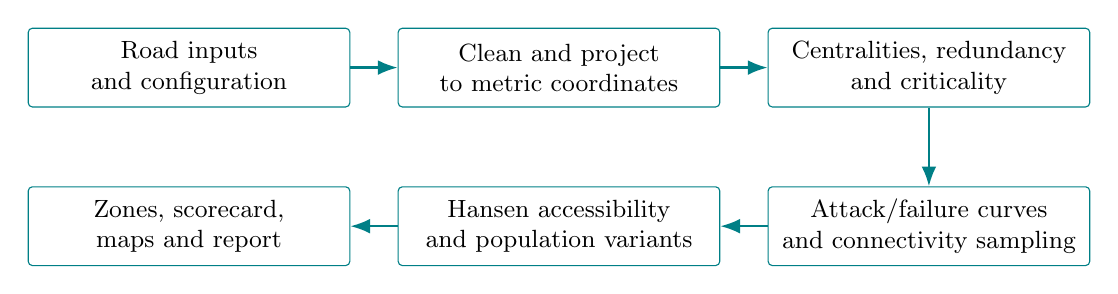
\begin{tikzpicture}[node distance=5mm and 6mm,
box/.style={draw=Teal,rounded corners=1.5pt,align=center,text width=3.85cm,minimum height=10mm,font=\small},
arr/.style={-{Latex[length=2.5mm]},thick,draw=Teal}]
\node[box] (input) {Road inputs\\and configuration};
\node[box,right=of input] (clean) {Clean and project\\to metric coordinates};
\node[box,right=of clean] (struct) {Centralities, redundancy\\and criticality};
\node[box,below=10mm of struct] (failure) {Attack/failure curves\\and connectivity sampling};
\node[box,left=of failure] (access) {Hansen accessibility\\and population variants};
\node[box,left=of access] (report) {Zones, scorecard,\\maps and report};
\draw[arr] (input)--(clean);\draw[arr] (clean)--(struct);\draw[arr] (struct)--(failure);
\draw[arr] (failure)--(access);\draw[arr] (access)--(report);
\end{tikzpicture}
\vspace{5mm}
\begin{itemize}\smallitems
\item Population changes the selected weights; zone polygons summarize finished results.
\item Seeds, parameters, data provenance and coverage are recorded with each run.
\end{itemize}
\src{Implementation: georesilience pipeline; Tickets 01--14. Boxes summarize dependencies rather than parallel execution.}
\end{frame}

% 08
\begin{frame}{Graph construction and cleaning}
\begin{itemize}\smallitems
\item Junctions become nodes; physical roads become links with metric length and geometry.
\item Simplification removes interstitial shape nodes; configurable intersection consolidation merges nearby junction representations.
\item Retain the largest component and report the nodes and road length discarded.
\item Use an undirected graph for structural centralities and directed paths for accessibility and default closure analyses.
\end{itemize}
\takeaway{Closing a two-way physical road removes both directed arcs together.}
\src{Tickets 01--03. Self-loops remain in exported layers but are excluded from analysis. Clipped boundaries can create artificial dead-ends.}
\end{frame}

% 09
\begin{frame}{Structural centrality and network classification}
\begin{columns}[T,totalwidth=\textwidth]
\column{.57\textwidth}
\small
\renewcommand{\arraystretch}{1.15}
\begin{tabular}{P{2.7cm}P{4.6cm}}
\toprule\textbf{Measure} & \textbf{Interpretation}\\\midrule
Degree & Local junction connections\\
Closeness & Distance to other nodes\\
Betweenness & Participation in shortest routes\\
Straightness & Euclidean distance relative to road distance\\
Information & Relative efficiency loss from isolating a node\\\bottomrule
\end{tabular}
\vspace{3mm}
\par\vspace{2mm}Classification compares distribution models. The nine-node grid is inconclusive (too few values).
\column{.39\textwidth}
\centering\img{edge_betweenness_map.png}{4.8cm}
\end{columns}
\src{Crucitti et al. (2006); Tickets 03, 05, 07. Map: local synthetic grid. Road degree alone does not determine the network class.}
\end{frame}

% 10
\begin{frame}{Redundancy and single-road criticality}
\begin{columns}[T,totalwidth=\textwidth]
\column{.49\textwidth}
\textbf{Screen every physical road}
\begin{itemize}\smallitems
\item Undirected bridges and articulation points
\item Directed endpoint detour ratio
\item Edge betweenness
\item Candidate selection plus analytic bridges
\end{itemize}
\column{.47\textwidth}
\textbf{Evaluate closure consequences}
\begin{itemize}\smallitems
\item Relative global-efficiency drop
\item Disconnected pair fraction
\item Extra distance for affected pairs
\item Population-weighted variants
\end{itemize}
\end{columns}
\vspace{2mm}
\[
\Delta E_e=\frac{E(G)-E(G\setminus e)}{E(G)},\qquad
E(G)=\frac{1}{N(N-1)}\sum_{i\ne j}\frac{1}{d_{ij}}
\]
\src{Tickets 04--05; Taylor et al. (2006) motivates consequence-based vulnerability. Infinite/unreachable distances contribute zero efficiency.}
\note{Explain that candidate-only rankings have a stated coverage. The controlled grid evaluates all 12 roads. The production efficiency uses inverse road distance, while the paper-reference comparison also considers spatial efficiency.}
\end{frame}

% 11
\begin{frame}{Cumulative attack and random failure}
\begin{columns}[T,totalwidth=\textwidth]
\column{.49\textwidth}
\textbf{Targeted attack}
\begin{itemize}\smallitems
\item Remove high-betweenness roads or nodes
\item Adaptive attack recomputes the ranking
\item Record cumulative damage at each step
\end{itemize}
\column{.47\textwidth}
\textbf{Random failure}
\begin{itemize}\smallitems
\item Remove randomly selected elements
\item Repeat with reproducible seeds
\item Report means and variation across runs
\end{itemize}
\end{columns}
\vspace{2mm}
Track largest strongly connected share $S(f)$ and relative efficiency $E(f)/E(0)$.
\[
\operatorname{AUC}(S)=\frac{1}{f_{\max}}\int_0^{f_{\max}}S(f)\,df
\]
\src{Albert et al. (2000); Ticket 06. The normalized AUC is a project summary, not the component fraction at the last removal step.}
\end{frame}

% 12
\begin{frame}{Connectivity reliability under uncertain closures}
\begin{itemize}\smallitems
\item Assign user-supplied per-event closure probabilities where available.
\item Otherwise use the length-scaled proxy $p_e=1-(1-p_0)^{L_e/(1\,\mathrm{km})}$.
\item Sample independent physical-road closures; recompute strongly connected components.
\item Average the mutually reachable pair fraction and retain sampling intervals.
\end{itemize}
\[
q=\frac{\sum_{c\in\mathrm{SCC}}n_c(n_c-1)}{N(N-1)}
\]
\takeaway{Pair connectivity, main-component membership and directed OD reachability are distinct.}
\src{Tickets 08--09; Taylor et al. (2006) motivates accessibility-based vulnerability. SCC aggregation and Monte Carlo design are project choices.}
\end{frame}

% 13
\begin{frame}{Distance-based accessibility and node vulnerability}
\begin{columns}[T,totalwidth=\textwidth]
\column{.5\textwidth}
\[
A_i=\sum_{\substack{j\ne i\\d_{ij}\le R}}W_j\exp(-\beta d_{ij})
\]
\small
\begin{itemize}\smallitems
\item $d_{ij}$: outbound directed road distance
\item $W_j=1$ or allocated destination population
\item $\beta=\ln 2/h$; inclusive cutoff $R=5h$ by default
\end{itemize}
\[
v_i=\max_{e\in\mathcal E_{\mathrm{evaluated}}}
\frac{A_i-A_i^{(-e)}}{A_i}
\]
\column{.46\textwidth}
\centering\img{hansen_decay.pdf}{4.5cm}
\end{columns}
\src{Ticket 11: the plan's truncated exponential Hansen definition. Plot: demo $h=100$ m, $R=500$ m. This differs from AP3's inverse-cost expression.}
\note{A is a sum of discounted opportunities, not a probability. Undefined A=0 origins do not receive a fabricated vulnerability of zero. Candidate coverage is reported. Optional k=2 is a top-three heuristic, not a global exhaustive search.}
\end{frame}

% 14
\begin{frame}{Population allocation and zone aggregation}
\begin{columns}[T,totalwidth=\textwidth]
\column{.49\textwidth}
\textbf{Population allocation}
\begin{itemize}\smallitems
\item Clip the count raster to the study boundary
\item Assign valid cell centres to the nearest analysis node
\item Apply a maximum snap distance
\item Report allocated and unallocated totals
\end{itemize}
\column{.47\textwidth}
\textbf{Zone aggregation}
\begin{itemize}\smallitems
\item Assign node points and road geometry midpoints
\item Sum population and physical-road length
\item Compute weighted means, coverage and ranks
\item Record unassigned features explicitly
\end{itemize}
\end{columns}
\takeaway{Population changes weights; zones never change routes, closures or network metrics.}
\src{Tickets 12--13. WorldPop is a modelled estimate. Entire road lengths follow their midpoint; zone density uses the full polygon area.}
\end{frame}

% 15
\begin{frame}{Population weighting represents different questions}
\small
\renewcommand{\arraystretch}{1.18}
\begin{tabular}{P{3.45cm}P{4.75cm}P{4.8cm}}
\toprule\textbf{Quantity} & \textbf{Weighting} & \textbf{Meaning}\\\midrule
Hansen $A_i$ and $v_i^{\mathrm{pop}}$ & Population weights destinations; origins averaged uniformly & Loss of access to population opportunities\\
Pair connectivity & Pair weight $w_iw_j$ & Expected connected share of population-product pairs\\
Population retained & Sum population in main SCC / allocated population & Expected share of allocated people in the largest node-count SCC\\
Zone-weighted vulnerability & $\sum_i w_i v_i/\sum_i w_i$ within a zone & Resident-weighted structural node loss\\
\bottomrule
\end{tabular}
\takeaway{The same population layer supports several measures with different denominators.}
\src{Tickets 09, 12--14. None of these weights represents observed trips or hospital demand. Main SCC is selected by node count with deterministic ties.}
\end{frame}

\section{Results}
% 16
\begin{frame}{Controlled example with independently known totals}
\begin{columns}[T,totalwidth=\textwidth]
\column{.46\textwidth}
\centering\img{presentation_population.pdf}{4.6cm}
\column{.5\textwidth}
\begin{itemize}\smallitems
\item $3\times3$ grid: \textbf{9 nodes, 12 physical roads}
\item Each road is 100 m; total road length \textbf{1.2 km}
\item Raster cell counts 1--9: \textbf{45 people-equivalent units}
\item West/East population: \textbf{27 / 18}
\item A third empty zone tests unavailable rankings
\end{itemize}
\end{columns}
\src{Local saved Ticket 14 demos. Synthetic population counts and polygons; these are not actual WorldPop observations or Hyderabad wards.}
\end{frame}

% 17
\begin{frame}{Connectivity survives while route efficiency falls}
\centering\img{robustness_links.pdf}{4.1cm}
\small
\begin{itemize}\setlength{\itemsep}{1.5mm}
\item After closing 2 of 12 roads, largest SCC share remains \textbf{1.0}.
\item Relative efficiency falls to \textbf{0.8729} under attack and \textbf{0.8951} under random failure.
\end{itemize}
\src{Local synthetic grid; 2 random-failure runs. Actual last removal is 16.67\%; dotted tails hold the last value to requested 20\% for AUC.}
\note{The small run illustrates a mechanism; it does not establish a city-wide robust-yet-fragile pattern. Connectivity AUC is 1 in both road cases, while efficiency AUCs are 0.9351 and 0.9434.}
\end{frame}

% 18
\begin{frame}{Population weighting changes road-criticality priorities}
\begin{columns}[T,totalwidth=\textwidth]
\column{.48\textwidth}
\centering\img{presentation_criticality.pdf}{4.6cm}
\column{.48\textwidth}
\small
\textbf{Top population-critical roads}
\par\vspace{3mm}
\renewcommand{\arraystretch}{1.2}
\begin{tabular}{rrr}\toprule
\textbf{Link ID} & \textbf{Uniform loss} & \textbf{Pop. loss}\\\midrule
\CriticalRows
\bottomrule\end{tabular}
\par\vspace{2mm}Individual-closure efficiency losses (percent).
\par\vspace{3mm}
These roads tie structurally, but population weighting separates their consequences.
\par\vspace{3mm}

\end{columns}
\src{Derived from the local saved physical-road layer. Colour scale is fractional efficiency loss; road labels are link IDs. Single closures, not simultaneous failure.}
\end{frame}

\begin{frame}{Population destinations change accessibility losses}
\begin{columns}[T,totalwidth=\textwidth]
\column{.60\textwidth}
\centering\img{accessibility_comparison.pdf}{4.6cm}
\column{.36\textwidth}
\small
\textbf{Mean worst-road loss}
\par\vspace{2mm}
Structural: \textbf{\MeanUniformLoss\%}
\par Population destinations: \textbf{\MeanPopulationLoss\%}
\par\vspace{4mm}
\textbf{All 12 roads evaluated}
\par $h=100$ m; $R=500$ m
\par\vspace{4mm}
Population changes the importance of destinations without changing the graph.
\end{columns}
\src{Local saved uniform/population summaries and node layers. These are deterministic closure losses for the controlled grid, not observed travel behaviour.}
\end{frame}

% 19
\begin{frame}{Vulnerable nodes retain geographic context}
\begin{columns}[T,totalwidth=\textwidth]
\column{.46\textwidth}
\centering\img{presentation_vulnerability.pdf}{4.6cm}
\column{.50\textwidth}
\begin{itemize}\smallitems
\item Structural vulnerability is highest at peripheral nodes in this grid.
\item Node-specific worst closures can differ across origins.
\item Population variants change which node/road receives priority.
\item Locator tables expose IDs, road names and WGS84 coordinates for inspection.
\end{itemize}
\end{columns}
\src{Map derived from the saved structural node layer; labels are node IDs. Population-destination top node is node 6, with loss 0.4286; see critical locator tables.}
\end{frame}

% 20
\begin{frame}{Reliability estimates depend on the closure model}
\small
\renewcommand{\arraystretch}{1.18}
\begin{tabular}{P{7.2cm}P{5.8cm}}
\toprule\textbf{Headline} & \textbf{Controlled-grid estimate}\\\midrule
Uniform mutual-pair connectivity & \UniformConnectivity\%\\
Population-product mutual-pair connectivity & \PopulationConnectivity\%\\
Allocated population retained in main SCC & \PopulationRetained\%\\
Expected allocated population cut off & \ExpectedCutOff\ out of 45 units\\
\bottomrule
\end{tabular}
\vspace{3mm}
\begin{itemize}\setlength{\itemsep}{2mm}
\item 1,024 samples; seed 42; independent physical-road failures.
\item $p_0=0.2$ is the 1 km proxy parameter: a 100 m road has $p_e\approx2.21\%$.
\item Uniform 95\% interval: $[0.998613,1]$; the high estimate reflects this graph and assumed probabilities.
\end{itemize}
\src{Local population summary.json. Sampling intervals are conditional on the chosen model; high observed reliability does not establish zero failure risk.}
\end{frame}

% 21
\begin{frame}{Zone results distinguish relative and absolute impact}
\begin{columns}[T,totalwidth=\textwidth]
\column{.55\textwidth}
\centering\img{zones_vulnerability_map.png}{4.4cm}
\column{.41\textwidth}
\small
\renewcommand{\arraystretch}{1.25}
\begin{tabular}{lrr}\toprule & \textbf{West} & \textbf{East}\\\midrule
Nodes & 6 & 3\\
Road km & 1.0 & 0.2\\
Population & 27 & 18\\
Weighted loss & \WestVuln\% & \EastVuln\%\\
Rank & 2 & 1\\\bottomrule
\end{tabular}
\par\vspace{2mm}
East has higher resident-weighted \emph{structural} loss.
\par\vspace{2mm}
Expected population cut off: West $0.010742$; East $0.008789$.
\end{columns}
\src{Local zones.gpkg and summary. Empty zone is unranked; no nodes/roads are unassigned. Synthetic geography; whole road lengths follow geometry midpoints.}
\end{frame}

% 22
\begin{frame}{The scorecard keeps the dimensions visible}
\begin{columns}[T,totalwidth=\textwidth]
\column{.65\textwidth}
\centering\img{scorecard_comparison.pdf}{4.6cm}
\column{.31\textwidth}
\small
\textbf{No default composite}
\par\vspace{3mm}
An explicitly weighted example gives
\par\vspace{2mm}
{\Large\bfseries\color{Teal}\ExampleComposite}
\par\vspace{3mm}
Example weights:
\par $0.3,0.1,0.1,$
\par $0.1,0.2,0.2$
\par\vspace{3mm}
Weights are disclosed and available scores are required.
\end{columns}
\src{Local Ticket 14 outputs; chart values are project normalisations. Composite uses the population run and is an illustrative choice, not a universal resilience rating.}
\end{frame}

% 23
\begin{frame}{Recorded real-data validation: central Mal\'e}
\begin{columns}[T,totalwidth=\textwidth]
\column{.58\textwidth}
\centering\img{male_allocation.pdf}{4.5cm}
\column{.38\textwidth}
\small
\begin{itemize}\smallitems
\item Actual OSM roads and Maldives WorldPop 2020 counts
\item \textbf{591 nodes; 951 roads}
\item \textbf{272 positive raster cells}
\item 100 m limit leaves 21 cells unallocated
\item Maximum nearest-node distance: \textbf{234.13 m}
\end{itemize}
\end{columns}
\src{Recorded 12 October 2026 validation in README/TICKET\_UPDATES; raw outputs absent locally. Same graph and settings; only snap limit changes.}
\note{Allocation was independently checked for every cell/node. Forty NetworkX Hansen checks had maximum absolute error 6.55e-11. This validates integration and arithmetic, not WorldPop census accuracy or Hyderabad coverage.}
\end{frame}

% 24
\begin{frame}{Recorded literature comparison preserves the mismatch}
\small
\renewcommand{\arraystretch}{1.18}
\begin{tabular}{P{2.7cm}P{1.3cm}P{4.1cm}P{4.7cm}}
\toprule
\textbf{City} & \textbf{Nodes} & \textbf{Expected information} & \textbf{Obtained information}\\\midrule
Ahmedabad & 2,870 & Power law & Power law\\
Cairo & 1,496 & Power law & Power law\\
Los Angeles & 240 & Exponential & Gaussian-like\\
Richmond, CA & 697 & Exponential & Gaussian-like\\
\bottomrule
\end{tabular}
\par\vspace{2mm}
\textbf{Information: 2/4 matches \qquad Betweenness: 3/4 matches}
\par\vspace{1mm}
\alert{MISMATCH}: at least 3/4 are required in each centrality.
\par\vspace{1mm}
Betweenness only mismatches Richmond: inconclusive in the framework and exponential in the reference.
\src{Recorded published-data Ticket 15, 11 October 2026; all 5,303 nodes evaluated. Both conventions agree on information; Gaussian-like means half-normal body preference.}
\end{frame}

% 25
\begin{frame}{Validation checks both arithmetic and complete runs}
\begin{columns}[T,totalwidth=\textwidth]
\column{.49\textwidth}
\textbf{Independent correctness checks}
\begin{itemize}\smallitems
\item Known-answer paths, cycles and bridges
\item NetworkX and exhaustive state references
\item Population conservation and nearest-node checks
\item Zone sums, weighted means and WGS84 locators
\end{itemize}
\column{.47\textwidth}
\textbf{Pipeline and output checks}
\begin{itemize}\smallitems
\item \textbf{341 passed, 5 skipped} in the full offline suite
\item Final focused suite: \textbf{42 passed}
\item Four local scenarios and an actual CLI run
\item Existing layers/results unchanged across Ticket 14
\end{itemize}
\end{columns}
\takeaway{Software correctness and geographic/model validity require different evidence.}
\src{Latest recorded regression and local verification files. Five skips are opt-in network/performance tests. Direct comparisons include population off/on.}
\end{frame}

\section{Observations}
% 26
\begin{frame}{Observations from the current evidence}
\begin{enumerate}\smallitems
\item \textbf{Connectivity alone misses route degradation.} The grid stays strongly connected while distance efficiency declines.
\item \textbf{Population changes the impact measure.} Mean worst-road loss rises from \MeanUniformLoss\% to \MeanPopulationLoss\% under population destinations.
\item \textbf{Relative and absolute zone priorities differ.} East ranks higher by weighted loss, while West has greater expected population cut off.
\item \textbf{A completed comparison can disagree with the paper.} Ticket 15 retains MISMATCH and inconclusive network labels.
\end{enumerate}
\src{First three observations concern the local synthetic grid. The fourth concerns recorded historical-city validation. Neither establishes a universal city ranking.}
\end{frame}

% 27
\begin{frame}{Limitations and current coverage}
\begin{itemize}\smallitems
\item Study boundaries and largest-component retention affect the available routes and population coverage.
\item Length proxies and independent closures represent assumptions; they are not calibrated flood probabilities or annual risk.
\item Candidate-only closure evaluation can understate the worst accessibility loss; the evaluated scope is reported.
\item WorldPop allocation is an estimate; ward means use assigned node population rather than a ward census.
\item Facilities, congestion and the full Hyderabad application are not demonstrated by the current controlled maps.
\end{itemize}
\src{Existing methodology limitations and coverage statements. Undefined metrics and skipped stages remain explicitly unavailable, rather than zero.}
\end{frame}

\section{Progress and future work}
% 28
\begin{frame}{Progress at mid-evaluation}
\small
\renewcommand{\arraystretch}{1.15}
\begin{tabular}{P{2.0cm}P{10.9cm}}
\toprule\textbf{Tickets} & \textbf{Implemented and tested capabilities}\\\midrule
01--05 & Inputs, cleaning, centralities, redundancy and single-road criticality\\
06--10 & Attack/failure, classification, probability inputs and reliability\\
11--12 & Hansen accessibility and population variants\\
13--14 & Zones, scorecard, final report and shared maps; both tickets committed\\
15 & Literature comparison and historical-data validation; MISMATCH retained\\
\bottomrule
\end{tabular}
\vspace{2mm}
End-to-end outputs: GIS layers, JSON metrics, reports, reproducible configuration and figures.
\src{TICKET\_UPDATES; commits 213acb5 and 1eafb90. Team manual review of the new zone/report outputs remains pending.}
\end{frame}

% 29
\begin{frame}{Next application and planned extensions}
\begin{columns}[T,totalwidth=\textwidth]
\column{.49\textwidth}
\textbf{Next application work}
\begin{itemize}\smallitems
\item Review the new zone/report outputs
\item Apply the framework to a frozen Hyderabad road extract, population and ward polygons
\item Examine coverage and parameter sensitivity
\item Investigate the recorded fitting discrepancy without tuning for agreement
\end{itemize}
\column{.47\textwidth}
\textbf{After the mid-evaluation}
\begin{itemize}\smallitems
\item Tier 3: essential facilities, service capacity and facility accessibility
\item Tier 4: travel demand, traffic assignment and calibrated delay
\item Optional: buffered boundaries and hazard-linked scenarios with justified data
\item Ticket 16: large-run execution/runbook
\end{itemize}
\end{columns}
\src{Existing proposal and design roadmap. These are future directions; facilities, traffic and calibrated flood scenarios are not current results.}
\end{frame}

% 30
\begin{frame}[fragile]{Demonstration: trace a result back to its data}
\begin{lstlisting}
georesilience run --config data/ticket14-demo/uniform.yaml
  --out results/mid-demo --overwrite
\end{lstlisting}
\small The command is one line when entered in the terminal.
\begin{enumerate}\smallitems
\item Inspect the scorecard and coverage warnings in \texttt{report.txt}.
\item Open node, road and zone layers in QGIS; locate a ranked feature by ID/coordinates.
\item Compare the uniform and population examples and inspect the zone totals.
\item Show a skipped/missing metric and the retained reason.
\end{enumerate}
\src{Saved outputs provide an offline fallback. Reproduce controlled population runs using examples/create\_ticket14\_demo.py, which freezes bbox acquisition.}
\note{Do not run population.yaml directly for the controlled demo: it downloads real OSM roads. Use the provided script for the frozen grid. The structural GraphML configuration runs offline.}
\end{frame}

% 31
\begin{frame}{References and evidence}
\small
\begin{itemize}\setlength{\itemsep}{3mm}
\item Albert, Jeong and Barab\'asi (2000). \emph{Error and attack tolerance of complex networks}. Nature 406, 378--382.
\item Crucitti, Latora and Porta (2006). \emph{Centrality measures in urban networks}. Physical Review E 73, 036125.
\item Taylor, Sekhar and D'Este (2006). \emph{Application of Accessibility Based Methods for Vulnerability Analysis of Strategic Road Networks}. Networks and Spatial Economics 6, 267--291.
\item Data: OpenStreetMap; WorldPop; authors' published historical city graphs.
\item Project evidence: proposal, design, implementation log, saved Ticket 14 outputs and independent verification files.
\end{itemize}
\src{Paper PDFs are included in the repository. Asset provenance and presentation chart sources are listed in asset\_sources.json in the LaTeX source package.}
\end{frame}

\appendix
\section{Technical appendix}
% 32
\begin{frame}{Appendix: centrality and criticality definitions}
\small
For connected metric graphs, closeness and straightness summarize distances:
\[
C_i^{\mathrm{close}}=\frac{N-1}{\sum_{j\ne i}d_{ij}},\qquad
C_i^{\mathrm{straight}}=\frac{1}{N-1}\sum_{j\ne i}\frac{d^{\mathrm{Euclidean}}_{ij}}{d_{ij}}.
\]
Betweenness counts participation in shortest paths; information measures the relative efficiency loss from isolating a node:
\[
C_i^{\mathrm{info}}=\frac{E(G)-E(G\setminus\mathrm{incident}(i))}{E(G)}.
\]
\begin{itemize}\setlength{\itemsep}{2mm}
\item Retain original $N$ after isolation; use metric road distances.
\item Framework efficiency: $\operatorname{mean}(1/d)$, units $\mathrm{m}^{-1}$.
\item AP2 reference: spatial efficiency $\operatorname{mean}(d^{\mathrm{Euclidean}}/d)$, dimensionless.
\end{itemize}
\src{Tickets 03, 05 and 15. These efficiency conventions answer different questions and are reported separately.}
\end{frame}

% 33
\begin{frame}{Appendix: population connectivity and uncertainty}
\small
For allocated node population $w_i$, the weighted mutually connected pair fraction in one sample is
\[
q_{\mathrm{pop}}=
\frac{\sum_c\left[(\sum_{i\in c}w_i)^2-\sum_{i\in c}w_i^2\right]}
{(\sum_iw_i)^2-\sum_iw_i^2}.
\]
Expected population cut off is a different measure:
\[
\mathbb E[P_{\mathrm{cut}}]=\sum_i w_i(1-p_i^{\mathrm{main\ SCC}}).
\]
\begin{itemize}\setlength{\itemsep}{2mm}
\item Network intervals average closure-sample fractions; node/OD intervals use Wilson estimates.
\item Intervals condition on the fixed model, inputs and selected origins where applicable.
\item Zero pair denominators are undefined; constant observed scores may miss rare failures.
\end{itemize}
\src{Tickets 09 and 12. The main SCC is the largest by node count, not necessarily by population.}
\end{frame}

% 34
\begin{frame}{Appendix: travel-time reliability is conditional on data}
\begin{columns}[T,totalwidth=\textwidth]
\column{.56\textwidth}
\small
\[
P\!\left(t_{ij}^{\mathrm{damaged}}\le(1+\tau)t_{ij}^{\mathrm{baseline}}\right)
\]
\begin{itemize}\smallitems
\item Default acceptable delay: $\tau=0.5$
\item Directed journeys from fixed sampled origins, plus supplied OD pairs
\item Replaceable additive time models; free-flow requires usable speed data
\item No usable speed data: explicit skip with a reason
\end{itemize}
\column{.40\textwidth}
\textbf{Current missing-data example}
\par\vspace{3mm}
\small Link robustness was not requested; tiny $R=0.5$ m makes accessibility undefined.
\par\vspace{3mm}
The report states \emph{not computed}; it does not turn missing scores into resilience of zero.
\end{columns}
\src{Ticket 10 and local missing-metrics scenario. Travel time is separate from distance Hansen accessibility and does not yet include congestion.}
\end{frame}

% 35
\begin{frame}{Appendix: scorecard normalisations and composite}
\small\renewcommand{\arraystretch}{1.07}
\begin{tabular}{P{5.4cm}P{7.6cm}}
\toprule\textbf{Dimension} & \textbf{Project-normalised score}\\\midrule
Attack / random-failure robustness & Corresponding normalized link $S$ AUC\\
Bridge redundancy & $1-\text{bridge count fraction}$\\
Detour redundancy & $1/\text{median finite detour ratio}$\\
Connectivity reliability & Expected mutual-pair fraction; population variant where defined\\
Accessibility retained & $1-\operatorname{mean}(v_i)$; destination-population variant where defined\\
\bottomrule
\end{tabular}
\vspace{2mm}
\[
C_{\mathrm{user}}=\sum_k\widetilde w_k s_k,\qquad
\widetilde w_k=\frac{w_k}{\sum_l w_l}
\]
\small No default weights; reject unknown keys or unavailable scores. Network class is unscored. Inverse detour can exceed one if an alternative is shorter.
\src{Ticket 14. These normalisations and weights are project reporting choices, not paper-defined universal resilience scores.}
\end{frame}

% 36
\begin{frame}{Appendix: interpreting the historical comparison}
\begin{itemize}\smallitems
\item The published four-city dataset preserves original topology, coordinates and metric road lengths.
\item Independent checks reproduce information scores to maximum error $3.30\times10^{-15}$ and planned-city betweenness to $2.78\times10^{-17}$.
\item Framework body fits and the AP2 reference use different model conventions; a relative fit preference is not absolute goodness of fit.
\item Ahmedabad spatial-information CCDF exponent: $2.7342$; Cairo: $2.6663$, compared with the paper's approximate $2.74$ and $2.63$.
\item Support, offsets and fitting ranges remain candidates for investigation; thresholds were not changed to force agreement.
\end{itemize}
\src{Recorded Ticket 15 published-data validation. CCDF exponent $\gamma=\alpha-1$ for an ideal continuous power-law density; exponent agreement is not the pass criterion.}
\end{frame}

% 37
\begin{frame}{Appendix: evidence locations and reproducibility}
\small
\renewcommand{\arraystretch}{1.15}
\begin{tabular}{P{3.5cm}P{9.5cm}}
\toprule\textbf{Evidence} & \textbf{Location / reproducibility}\\\midrule
Local runs & \texttt{results/ticket14-demo/}: uniform, population, user-weighted, missing-metrics\\
Independent checks & \texttt{verification.json}; \texttt{backward\_compatibility.json}\\
Raw spatial results & Each run's \texttt{network.gpkg} and optional \texttt{zones.gpkg}\\
Recorded earlier runs & Real Mal\'e and published-city results in README and TICKET\_UPDATES\\
Tests & Full offline suite: 341 passed, 5 skipped; final focused checks: 42 passed\\
Slide data & \texttt{build\_assets.py}, \texttt{results\_macros.tex}, \texttt{asset\_sources.json}\\
\bottomrule
\end{tabular}
\vspace{3mm}
\small Figures reuse saved outputs or labelled records; slide creation runs no new network analysis.
\src{Local chart sources are tracked with hashes. The LaTeX package contains all figures required to rebuild the PDF.}
\end{frame}

\end{document}
